\begin{frame}{How to integrate FAIR concepts in my work ?}{Some tools for reproducible research}
\begin{itemize}
\item {\sout{\color{gray} FAIR apply on the data}}
\item FAIR apply to the code
\end{itemize}
\begin{textblock*}{15cm}(5cm,1.5cm) % {block width} (coords)
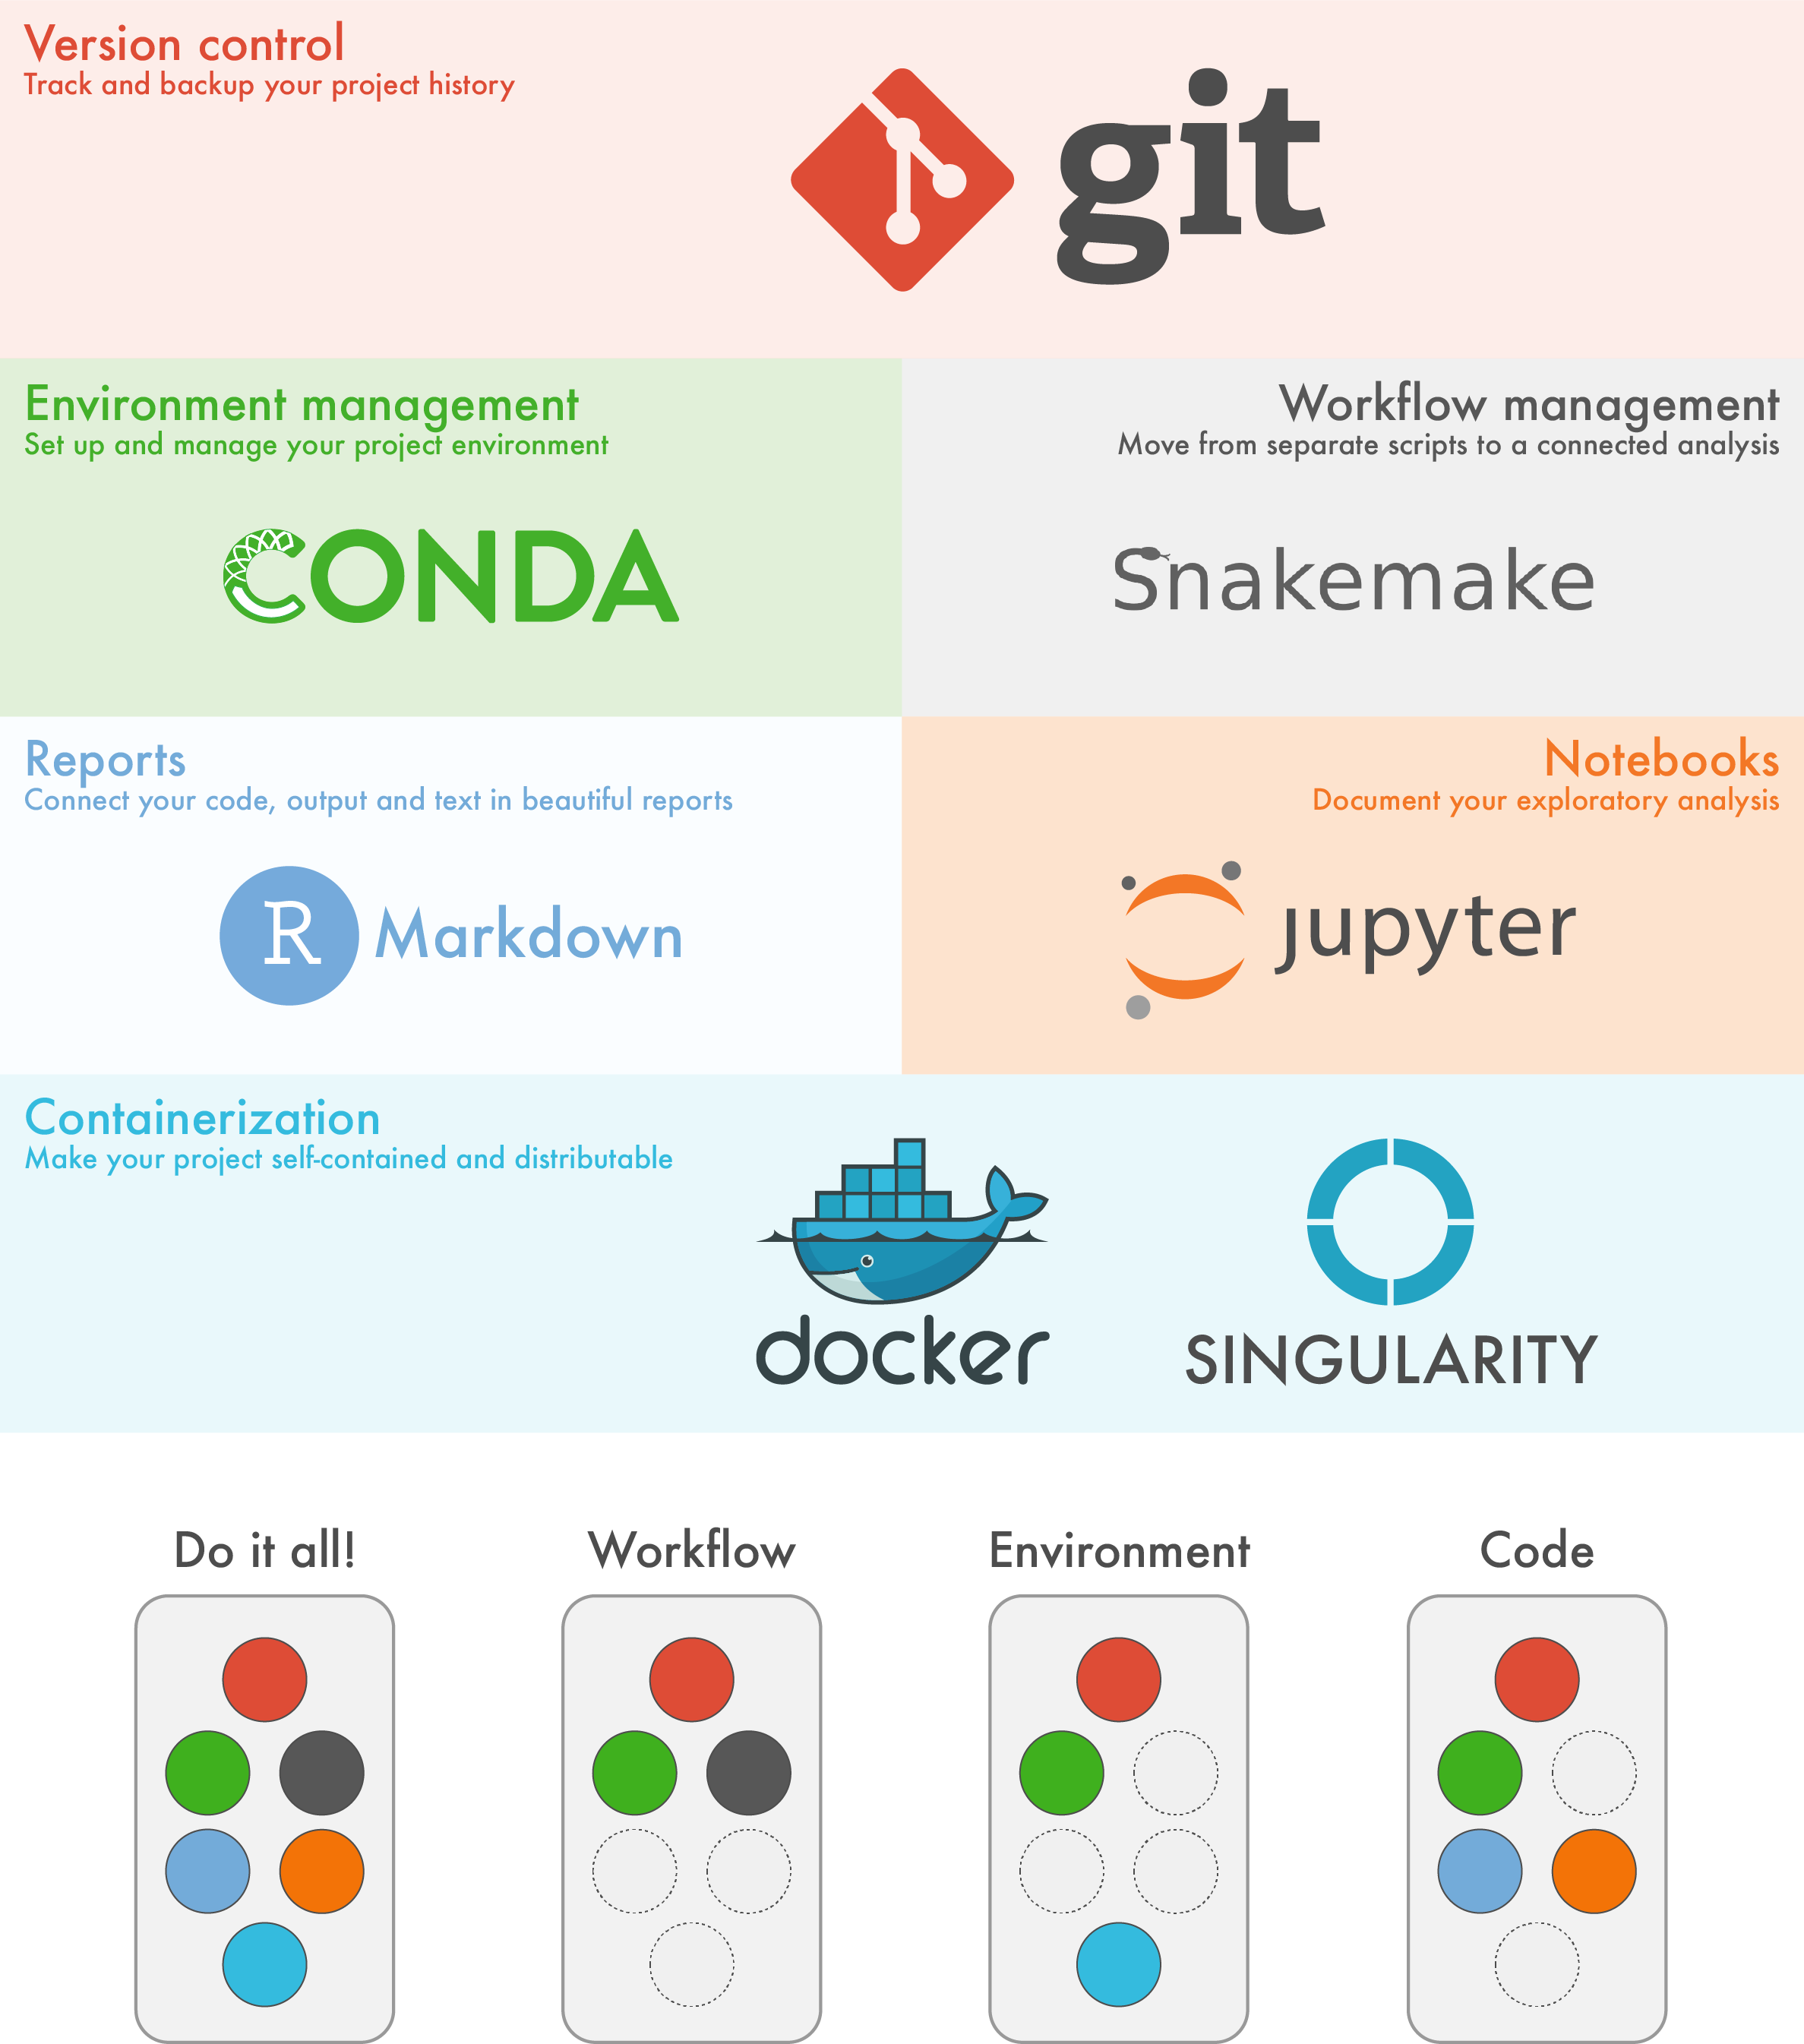
\includegraphics[scale=0.3]{tutorials_overview.png}
\end{textblock*}
\end{frame}

\begin{frame}{FAIR session with AuBi}
\begin{block}{Objectives}<1->
\begin{itemize}
\item Discover FAIR practices
\item Discover tools for best practices
\item Learn tools and best practices
\item<2-> 5 sessions for courses and practices
	\begin{itemize}[<2->]
	\item Day 1: Introduction to FAIR and building training environment
	\item Day 2: Code versioning with Git
	\item Day 3: Environment managment using conda and docker/singularity
	\item Day 4: Workflow managment using snakemake
	\item Day 5: Documentation using Rmarkdown or Jupyter
	\end{itemize}
\end{itemize}
\end{block}
\end{frame}

\section{Training content}
\begin{frame}
\begin{block}{Contents}
\begin{itemize}
\item<1-> Introduction to FAIR practices
\item<2-> Code control using Git \faGit* 
	\begin{itemize}[<2->]
	\item Git environment
	\item Gitlab and Github \faGithub \faGitlab
	\end{itemize}
\item<3-> Encapsulation process
	\begin{itemize}[<3->]
	\item Conda environment and packages use 
\includegraphics[scale=0.07]{conda_logo.pdf}
	\item Containers as docker \& singularity \faDocker 
	\item Reproducible workflow using snakemake 	
\includegraphics[scale=0.05]{snakemake_logo.png}
	\end{itemize}
\item<4-> Literate programming and documentation
	\begin{itemize}[<4->]
	\item Markdown syntax \faMarkdown
	\item Rmarkdown for R \faRProject 
	\item Jupyterlab for Python \faPython
	\end{itemize}
\end{itemize}
\end{block}
\end{frame}